\begin{center}
  \normalsize{\cyr{\textbf{№3.7}}}
\end{center}

\begin{figure}[h!]
  \centering
  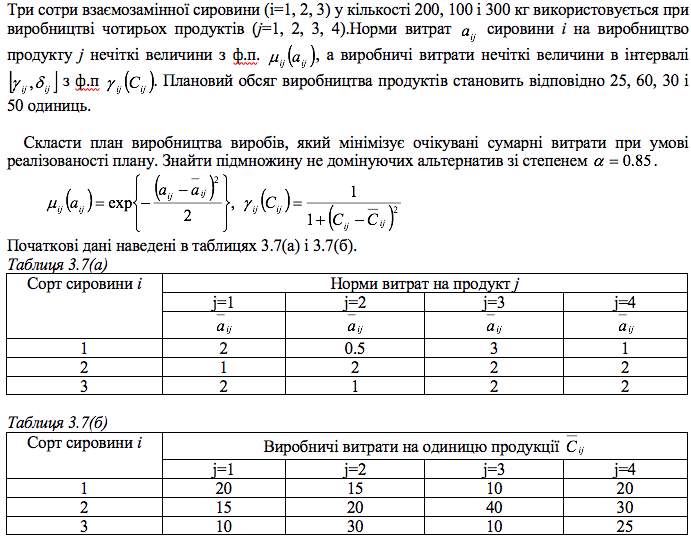
\includegraphics[width=11.2cm]{3_7.png}
  \centering
\end{figure}


Математична модель: $x_{ij}$ продукт $j$ з сировини $i$
$$
min \qquad   \sum_i^3\sum_j^4 C_{ij} x_{ij}
$$
\Title{Обмеження}
\Code {\sum_i^3 a_{ij} x_{ij} \leqslant b_i \qquad \sum_j^4  x_{ij} \geqslant P_j }

\begin{multicols}{2}
  $$\mu(a_{ij}) \geqslant 0.85  $$

  $$ \exp\{ - \dfrac{(a_{ij}-\overline{a}_{ij})^2}{2} \} \geqslant 0.85 $$

  $$- \dfrac{(a_{ij}-\overline{a}_{ij})^2}{2} \geqslant \ln{0.85} $$

  $$ (a_{ij}-\overline{a}_{ij})^2 \leqslant -2 \ln{0.85} $$

  $$ (a_{ij}-\overline{a}_{ij})^2 \leqslant 2 \ln{\dfrac{20}{17}} $$


  $$|a_{ij}-\overline{a}_{ij}| \leqslant \sqrt{2\ln{\dfrac{20}{17}}} $$

  $$ a_{ij} - \sqrt{2 \ln{\dfrac{20}{17}}} \leqslant a_{ij} \leqslant a_{ij} + \sqrt{ 2 \ln{\dfrac{20}{17}}}$$

  \columnbreak
  $$\gamma(C_{ij}) \geqslant 0.85 $$

  $$
  \dfrac{1}{1+(C_{ij}-\overline{C}_{ij})^2} \geqslant 0.85
  $$

  $$
  \dfrac{1}{0.85} \geqslant 1+(C_{ij}-\overline{C}_{ij})^2
  $$

  $$
  \dfrac{1}{0.85} - 1 \geqslant (C_{ij}-\overline{C}_{ij})^2
  $$

  $$
  \dfrac{3}{17} \geqslant (C_{ij}-\overline{C}_{ij})^2
  $$

  $$
  \sqrt{\dfrac{3}{17}} \geqslant |C_{ij}-\overline{C}_{ij}|
  $$

  $$
  C_{ij} - \sqrt{\dfrac{3}{17}} \leqslant C_{ij} \leqslant C_{ij} + \sqrt{\dfrac{3}{17}}
  $$

\end{multicols}

\begin{multicols}{2}


  \Title{Задача песиміста}

  \Code{
    min \quad \sum_i^3\sum_j^4( \overline{C}_{ij}  + \sqrt{\dfrac{3}{17}}) x_{ij}
  }

  \Title{Обмеження}

  \Code{
  \sum_i^3( \overline{a}_{ij} + \sqrt{ 2 \ln{\dfrac{20}{17}}} ) x_{ij} \leqslant b_i
  }
  \Code { \sum_j^4  x_{ij} \geqslant P_j }

  \columnbreak

  \Title{Задача оптиміста}


  \Code{
    min \quad \sum_i^3\sum_j^4( \overline{C}_{ij} - \sqrt{\dfrac{3}{17}}) x_{ij}
  }

  \Title{Обмеження}

  \Code{
    \sum_i^3( \overline{a}_{ij} - \sqrt{ 2 \ln{\dfrac{20}{17}}} ) x_{ij} \leqslant b_i
  }
  \Code { \sum_j^4  x_{ij} \geqslant P_j }

\end{multicols}
